\section{Projektstrukturplan}

\subsection{Zielbestimmung}
\subsubsection{Musskriterien}
Diese Kriterien müssen bis zum Projektende implementiert werden, damit das Projekt erfolgreich abgeschlossen ist.

\begin{description}
	\item[/MK10/] Die zu lernenden Karten werden durch einen Algorithmus ausgewählt (z.B. Leitner System)
	\item[/MK20/] Unicode-Zeichen werden als Eingabe in den Karteikarten unterstützt.
	\item[/MK30/] Bilder können eingefügt werden.
	\item[/MK40/] Ein Karteikartenset kann vom Benutzer exportiert werden.
	\item[/MK50/] Ein (anderer) Benutzer kann das vom \textbf{/MK40/} exportierte Karteikartenset für seinen Account importieren.
	\item[/MK60/] Die Seite stellt ein Katalog von vorgefertigten Karteikartensets zur Verfügung.
	\item[/MK70/] Der Benutzer hat Option ein Karteikartenset mit einer anderen Person zu teilen.
	\item[/MK80/] Beim Lernen mit den Karteikarten kann auch nur mit der Tastatur navigiert werden.
\end{description}

\subsubsection{Wunschkriterien}
Diese Kriterien werden für das Projekt gewünscht, sind aber nicht zwingend erforderlich für ein erfolgreiches Projektende. Je nach Zeit und technisches Schwierigkeitsgrad wird versucht möglichst viele/wichtige Kriterien zu implementieren.

\begin{description}
	\item[/WK10/] Die Webseite wird zusätzlich auch für Mobilgeräte optimiert.
	\item[/WK20/] Für jedes Karteikartenset werden Statistiken angezeigt (Erfolgsquote,...).
	\item[/MK30/] Mathematische Ausdrücke werden dargestellt in natürlicher Form (z.b. \( e^{\frac{3}{4}\pi i}\))
	\item[/MK40/] Die Antwortkarte kann in Form von Multiple Choice sein.
\end{description}

\subsubsection{Abgrenzkriterien}
Diese Kriterien beschreiben die Grenzen des Projektes und sollen auf jeden Fall nicht implementiert werden.
\begin{description}
	\item[/AK10/] Videos müssen nicht in die Karten eingebettet sein. (Sie können trotzdem einfach als Hyperlink eingefügt werden.)
	\item[/AK20/] Die Webseite muss nicht offline funktionieren.
	\item[/AK30/] Bei Verbindungsverlust muss der aktuelle Stand nicht zwischengespeichert werden.
\end{description}

\subsection{Produkteinsatz}
% in diesem Kapitel kann der Einsatz auch eingegrenzt werden

\subsubsection{Anwendungsbereiche}

\subsubsection{Zielgruppen}
\begin{description}
	\item[/A10/] Die Webseite richtet sich an Personen, die eine neue Fremdsprache lernen wollen.
	\item[/A20/] Eine weitere Zielgruppe sind Schüler, die die Webseite begleitend zum Unterricht benutzen.
	\item[/A30/] Die letzte Gruppe sind Studenten, die die Webseite begleitend zum Studium benutzen.
\end{description}

\subsubsection{Betriebsbedingungen}
Die Betriebsbedingungen beschreiben die physikalische Umgebung und tägliche Betriebszeit. ständige Beobachtung oder unbeaufsichtigter Betrieb

\subsection{Produktübersicht}

\subsection{Produktfunktionen}

\subsection{Produktdaten}
\subsubsection{Benutzer}
Zu dem angemeldeten Benutzer werden diese Daten dauerhaft gespeichert:
\begin{itemize}
	\item Benutzername
	\item E-Mail-Adresse
	\item Password
\end{itemize}

\subsubsection{Lernkartei}
Für jede einzelne Lernkartei werden diese Informationen gespeichert:
\begin{itemize}
	\item Inhalt der Frage
	\item Inhalt der Antwort
	\item Anzahl der richtigen und falschen Beantworten der Frage
	\item Zeitpunkt der letzten richtigen Beantwortung der Frage
\end{itemize}

\subsection{Produktleistungen}

\section{Nichtfunktionale Anforderungen}
Diese Anforderungen befassen sich nicht nicht mit der Funktionalität des Projektes, sondern mit anderen Themen wie z.B. Qualität, Schnelligkeit und Benutzerfreundlichkeit. Auch rechtliche Anforderungen können hier beschrieben werden.

\subsection{Qualität}
\begin{description}
     \item[/NF10/] Die Webseite soll die Musskriterien erfüllen.
     \item[/NF20/] Die Webseite soll möglichst unbeaufsichtigt betrieben werden können.
     \item[/NF30/] Das Lernen der Karteikarten soll möglichst einfach sein.
     \item[/NF40/] Fehler ausgelöst durch den Benutzer soll abgefangen werden und wenn nötig durch eine Fehlermeldung angezeigt werden.
     \item[/NF50/] Die Seite soll ein Stresstest mit 300 registrierten Benutzern und 200 Aufrufe in der Minute aushalten.
\end{description}

\subsection{Getestete Browser}
\begin{itemize}
	\item Google Chrome (ab Version ...)
	\item Mozilla Firefox (ab Version ...)
	\item Internet Explorer (ab Version ...)
	\item Apple Safari (ab Version ...)
	\item Google Chrome for Android (ab Version ...)
	\item Apple Safari for iPad (ab Version ...)
\end{itemize}

\subsection{Rechtliche Informationen}
Das Produkt ist quelloffen und wird nichtkommerziell unter der freien "GNU General Public Licence"-Lizenz zur Verfügung gestellt. Dies ist mit allen verwendeten Bibliotheken und Tools vereinbar.

\section{Globale Testfälle}
Dies sind einige Testfälle, die die korrekte Ausführung verschiedener Funktionen überprüfen.

\subsection{Testfälle für Pflichtkriterien}
\begin{description}
	\item[/TP10/] Ein korrekt-beantwortete Karte sollte beim wiederholten Lernen kurz danach (in Abhängigkeit vom Algorithmus) nicht auftauchen.
	\item[/TP20/] Seltene Unicode-Zeichen wie \(\pi\) werden als Eingabe benutzt und danach im Lernmodus überprüft.
	\item[/TP30/] Ein Bild wird als Eingabe benutzt und danach im Lernmodus überprüft.
	\item[/TP40/] Ein Karteikartenset wird exportiert und danach wird getestet, ob die Datei auch übereinstimmt.
	\item[/TP50/] Das von \textbf{/TP40/} exportierte Karteikartenset wird importiert.
	\item[/TP60/] Ein im Katalog vorgefertigte Karteikartenset wird zum eigenen Account hinzugefügt.
\end{description}

\section{Benutzeroberfläche}
\subsection{Hauptbildschirm}

\begin{figure}[H]
    \centering
    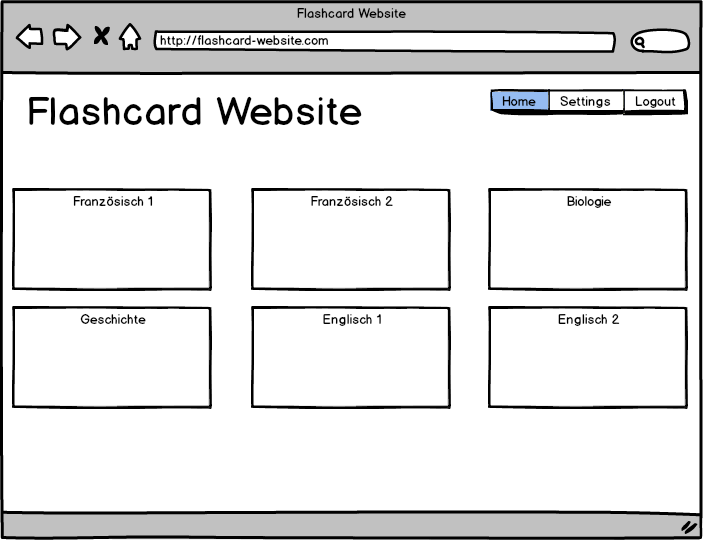
\includegraphics[width=0.7\textwidth]{images/Overview.png}
    \caption{Hauptbildschirm}
    \label{fig:overview}
\end{figure}

Der Hauptbildschirm gibt eine Übersicht zu den Karteikartensets des angemeldeten Benutzers. Beim Klicken auf eines der Sets kommt man zum Lernbildschirm


\subsection{Lernbildschirm}


\begin{figure}[H]
    \centering
    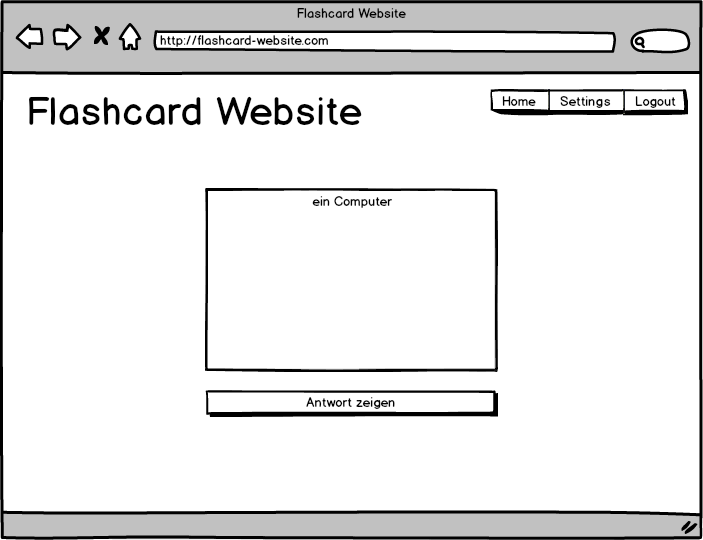
\includegraphics[width=0.7\textwidth]{images/Lernscreen-Frage.png}
    \caption{Frageseite einer Karteikarte}
    \label{fig:lernscreen-frage}
\end{figure}

\begin{figure}[H]
    \centering
    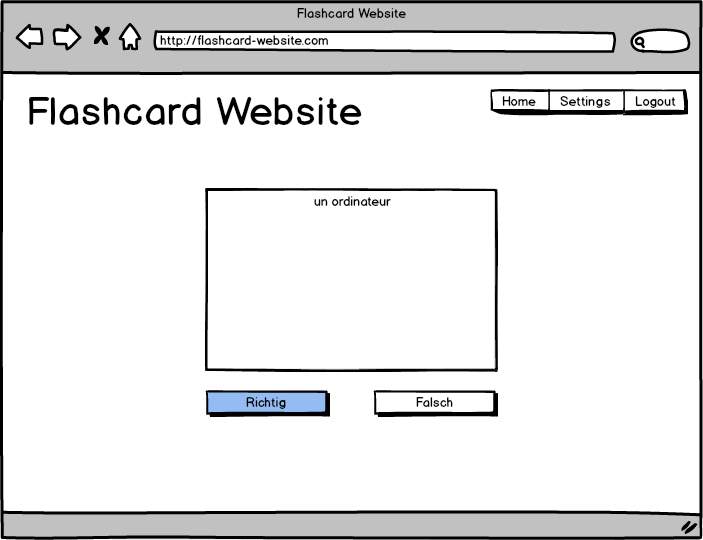
\includegraphics[width=0.7\textwidth]{images/Lernscreen-Antwort.png}
    \caption{Antwortseite einer Karteikarte}
    \label{fig:lernscreen-antwort}
\end{figure}

Der Lernbildschirm fängt mit der Vorderseite von der ersten Karteikarte des Sets an. Wenn man sich die Rückseite mit der Antwort anzeigen lässt, hat man die Möglichkeit anzugeben, ob man richtig lag oder nicht.

\begin{figure}[H]
    \centering
    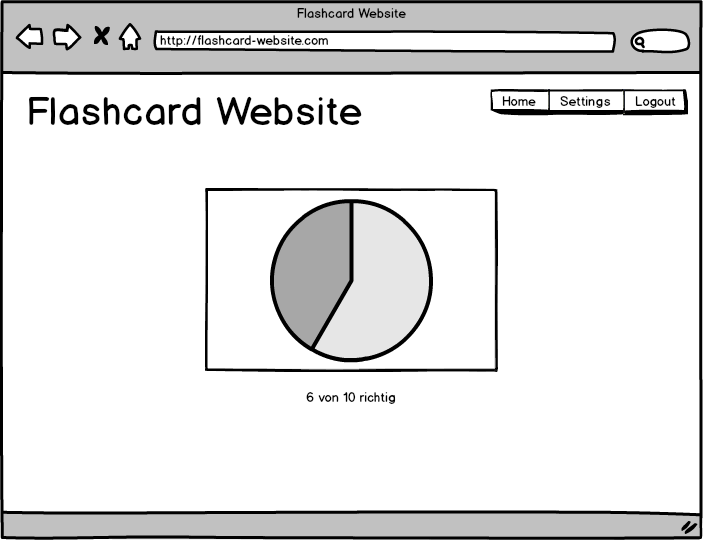
\includegraphics[width=0.78\textwidth]{images/Lernscreen-Ergebnis.png}
    \caption{Ende des Karteikartensets}
    \label{fig:lernscreen-ergbenis}
\end{figure}

Nachdem man alle Karteikarten durchgegangen ist, wird eine Statistik zu der Anzahl an richtigen Antworten angezeigt.
